% macro for the title of this doc.
\newcommand{\documentName}{Software Design Document}
\newcommand{\shortDocumentName}{SDD}

% include the macros from docs/project_macros.tex
% use %input{../defines.tex} to include these.
% This document contains all of the common macros and setup across documents.

% %%%%%%%%%%%%%%%%%%%%%%% Start Update lines %%%%%%%%%%%%%%%%%%%%%%%%%%%%
% These are the lines to update to change the versions in all documents.
% currentVersion is the current version of the document.
% longDate is the long date the documents were updated at.
% firstDraftLine, snapshotOneLine, snapshotTwoLine, etc
% are the revision history table lines.
% %%%%%%%%%%%%%%%%%%%%%%%%%%%%%%%%%%%%%%%%%%%%%%%%%%%%%%%%%%%%%%%%%%%%%%%

% Update this to update the current versions.
\newcommand{\currentVersion}{1.1.0}

% update this to change the date on the documents.
\newcommand{\longDate}{November 19, 2026}

% Update these to add each version
% every row must end with '\\ \hline'
\newcommand{\firstDraftLine}{%
Project Group 26 & 11/17/2026 & First Draft & 1.0.0 \\ \hline
}
\newcommand{\snapshotOneLine}{%
Project Group 26 & 11/19/2026 & Snapshot 1 update & 1.1.0 \\ \hline
}
\newcommand{\snapshotTwoLine}{}
\newcommand{\snapshotThreeLine}{}
\newcommand{\snapshotFourLine}{}
%%%%%%%%%%%%%%%%%%%%%%%% End Update lines %%%%%%%%%%%%%%%%%%%%%%%%%%%%%%


% We expect \newcommand{\documentName}{User Manual} to define the name of this document.
% We fill in the titles from that.
\newcommand{\myTitle}{Golden Eagle Flight Plan \documentName}
\newcommand{\longTitle}{Golden Eagle Flight Plan\\\documentName\\CS 3338 Final Project}


\documentclass[11pt,letterpaper]{article}
\usepackage[margin=1in]{geometry}
\usepackage[T1]{fontenc}
\usepackage[utf8]{inputenc}
\usepackage{lmodern}
\usepackage{longtable,booktabs,array,enumitem,hyperref,xcolor,graphicx,pdflscape}
\usepackage{indentfirst}
\usepackage{fancyhdr}
\usepackage{graphicx}
\usepackage{titling}
\usepackage{enumitem}
\usepackage{amssymb}
\hypersetup{colorlinks=true,linkcolor=blue,urlcolor=blue}
\setlist[itemize]{leftmargin=*}

% Automatically prefixes the section number to all first-level enumerate lists
% label=\thesubsection.\arabic* pulls "1.1" and adds the list item number
% leftmargin=3\parindent indents 3 paragraphs.
\setlist[enumerate,1]{label=\thesubsection.\arabic*,leftmargin=\parindent}

\newlist{subenumerate}{enumerate}{2}
\setlist[subenumerate,1]{label=\thesubsubsection.\arabic*,leftmargin=\parindent}

\pagestyle{fancy}
\geometry{a4paper, margin=1in}

% Create a todo list
\newlist{todolist}{enumerate}{2}
\setlist[todolist]{label=\thesection.\arabic*,leftmargin=\parindent}
\usepackage{pifont}
\newcommand{\cmark}{\ding{51}}%
\newcommand{\xmark}{\ding{55}}%
% Each marker draws the single checkbox for its item.
\newcommand{\planned}{\leavevmode$\square$\ \textit{(still to be confirmed)}\ }
\newcommand{\done}{\leavevmode\rlap{$\square$}\hspace{1pt}\cmark\ \ }
\newcommand{\wontfix}{\leavevmode\rlap{$\square$}\hspace{1pt}\xmark\ \ }

\newcommand{\authors}{Project Group 26\\Jason Reese \\ Juan Torres Llamas \\ Victor Hernandez}



% First PageBlock.
% This section makes the First Page, Revision Table and TOC match across all documents.
% Prefixing an argument with + makes it "long," 
% it expects the 
% allowing it to accept multi-paragraph blocks, lists, and display math.
\NewDocumentCommand{\firstPageBlock}{}{%
\title{\longTitle}

\fancyhf{}
\pagestyle{fancy}
\fancyhead[L]{\myTitle}
\fancyhead[R]{Page \thepage}
\fancyfoot[C]{}

\newpage %


\author{Project Group 26\\Jason Reese \\ Juan Torres Llamas \\ Victor Hernandez}
\date{\longDate}

\newpage %
\maketitle

\newpage %

\begin{table}[h!]
\centering
\caption{\textbf{Revision History}}
\begin{tabular}{|c|c|c|c|}
\hline
\textbf{Name} & \textbf{Date} & \textbf{Reasons for Changes} & \textbf{Version} \\
\hline
\firstDraftLine
\snapshotOneLine
\snapshotTwoLine
\snapshotThreeLine
\snapshotFourLine
\end{tabular}
\end{table}
\newpage %

\begin{center}Design draft --- November 2026\end{center}
\tableofcontents
\newpage %

}


\begin{document}

\firstPageBlock

\newpage %
\section{Introduction}
\subsection{Purpose}
The Golden Eagle Flight Plan is an application that helps university students track their four-year academic and professional development journey in one centralized platform.
Currently, students must juggle multiple disconnected sources for campus resources and advising: emails, social media, various websites, and one-off meetings with advisors.
This application solves that problem by bringing everything together: a gamified scoreboard system that tracks student progress across Academic Preparation, Career
Development, and Community \& Leadership; a personalized resources and events feed that surfaces content relevant to each student's major, year, and interests; and a faculty-
facing dashboard that allows advisors to post targeted content and monitor individual student progress. The goal is to graduate well-rounded, career-ready, and community-
engaged students by making growth visible and actionable for both students and faculty.

% Start the Document Conventions Subsection.
\documentConventionsBlock{The design is based on \emph{SRS v\currentVersion} and \emph{PDS v\currentVersion}}

\subsection{Intended Audience and Reading Suggestions}
Readers of this document should be familiar with the overall project design \emph{Project Design Specification v\currentVersion} and the project requirements\emph{SRS v\currentVersion}.

\subsection{System Overview}
The System is comprised of a Front End which is the website that the users interact with, a Back End which the Front End accesses in order to update and retrieve details and a Database that stores all of the relevant information.

\subsubsection{Front End}
The front end is written in JavaScript, CSS, and HTML and displayed in the users browser.
It makes API calls to the back end in order to authenticate, and display details to the user for any page they wish to visit.

\subsubsection{Back End}
The back end is written in JavaScript running on Node.js, and interacts with the Postgres Database for storage. It contains all of the business logic for the application.

All api calls to the backend must be authenticated.

The only calls that do not require authentication are the Unauthenticated Endpoints listed in the Back End Design section.

\newpage %
\section{Design Considerations}
    \subsection{Assumptions and Dependencies}
        \begin{itemize}[leftmargin=3\parindent]
            \item Users have basic knowledge to navigate websites.
            \item Users have a working internet connection.
            \item The software will change as features are added.
        \end{itemize}

    \subsection{General Constraints}
    Security and Privacy constraints require that all calls be authenticated, and that passwords are only transmitted over HTTPS.

    The site must be accessible on limited bandwidth and screen size constrained devices.

    \subsection{Technical Constraints}
    All API calls must be authenticated, which will require the login process to store limited data on in the browser in order for the site to function.

    Passwords must only be sent to the backend over HTTPS, and must never be logged or stored in plain text.

    In order to leverage the Cal State LA Single Sign On, there will be changes made depending on the technologies Cal State SSO leverages.

    \subsection{Risks}
        \begin{enumerate}[leftmargin=3\parindent]
            \item \textbf{First Administrator takeover.} The first user to create an account becomes the Admin user, so if a new deployment is reachable before its owner creates the first account, anyone who finds it can create the first account and gain full control of the site.
                \begin{itemize}
                    \item \textit{Impact:} The attacker would have all permissions, including approving accounts, viewing student profiles, and managing roles, and the owner would have to reset the database to recover.
                    \item \textit{Mitigation:} The first account must be created before the site is made publicly available. This can be done with a first time setup script that creates the Admin user directly in the database before deployment, so that the site never starts without an Admin. The creation is recorded in the Security Event table so it can be reviewed. A stronger option, such as a one-time setup token supplied at install time, can be added if this risk is not acceptable.
                \end{itemize}
        \end{enumerate}

\newpage %
\section{Front End Design}
The front end consists of the user visible web pages.
The content of all pages will be fetched from the backend and displayed to the user.

All requests to the backend must contain an authorization cookie that can be linked back to the user request.

Upon a successful login the backend will return a JWT to the user that can be used to authenticate all future back end calls, and can be refreshed.

Security best practices will be followed including leveraging CORS, CSRF and anti-replay.

\subsection{Login Page Design}
    \subsubsection{Login Page}
        \begin{enumerate}[leftmargin=3\parindent]
            \item If the user is not logged in they will be redirected to a login page upon attempting to access any part of the site.
            \item The login page will have two buttons:
                \begin{itemize}
                    \item A button for logging into an existing account.
                    \item A button for creating a new account.
                \end{itemize}
        \end{enumerate}
    \subsubsection{Logging Into an Existing Account}
        \begin{enumerate}[leftmargin=3\parindent]
            \item If the user decides to log into an existing account, they will be redirected to a page where they can enter their username and password in two different text fields.
            \item The username field will be above the password field and both fields will be labeled.
            \item There will be a forgot password button below the password field.
            \item Underneath the forgot password button will be a login button.
            \item The password field will be censored and each character the user enters into the field will appear as a \textbullet\ to the user.
            \item If the user clicks the login button, the site will first check if the username is present in the database. If it is, it will confirm if the passwords match.
            \item If the username isn't in the database or the passwords don't match, the user will stay on the login screen and will be prompted with an error telling them Incorrect Username/Password.
            \item The error will not tell the user which was incorrect, only that one of the two was incorrect.
            \item If the user is able to successfully login, they will be redirected to the homepage.
        \end{enumerate}
    \subsubsection{Forgot Password}
        \begin{enumerate}[leftmargin=3\parindent]
            \item If the user clicks the forgot password button, they will be redirected to a screen that tells the user a link to reset the password has been sent to the email associated with the account.
            \item The confirmation screen should not tell the user what email it was sent to.
            \item The link in the email will redirect the user to a reset password screen in which they will enter their new password and confirm their new password.
            \item A Forgot Password request should expire all existing JWTs.
        \end{enumerate}
    \subsubsection{Creating a New Account}
        \begin{enumerate}[leftmargin=3\parindent]
            \item If the user decides to create a new account, they will be redirected to a page in which they click on one of three buttons that determine whether they are trying to create a Student, Faculty, or Student Organization account.
            \item If the user clicks the student option they will be asked to enter the following information in different text fields:
                \begin{itemize}
                    \item First Name
                    \item Last Name
                    \item Username
                    \item Password
                    \item Confirm password
                    \item University Email Address
                    \item Major
                    \item Phone number
                \end{itemize}
            \item If the user clicks the faculty option they will be asked to enter the following information in different text fields:
                \begin{itemize}
                    \item First Name
                    \item Last Name
                    \item Username
                    \item Password
                    \item Confirm password
                    \item University Email Address
                    \item Phone number
                    \item Department
                    \item Job Title
                \end{itemize}
            \item If the user clicks the student organization option they will be asked to enter the following information in different text fields:
                \begin{itemize}
                    \item Organization name
                    \item Username
                    \item Password
                    \item Confirm password
                    \item Email Address
                    \item Description of the organization
                \end{itemize}
            \item The password and confirm password text fields will be censored and each character the user enters into the field will appear as a \textbullet\ to the user.
        \end{enumerate}
    \subsubsection{Account Validation}
        \begin{enumerate}[leftmargin=3\parindent]
            \item The user will not be able to create an account using an email that is already present in the system.
            \item The system will reject any email addresses that are entered and do not end in \emph{@calstatela.edu} for \emph{Student} or \emph{Faculty}.
            \item The system will accept any email address for \emph{Student Organization}.
            \item If the user claims to be a \emph{Faculty} or \emph{Student Organization}, the account will be created as pending and inactive, and they will be redirected to a site telling them their account will be activated once an Administrator approves it.
            \item A pending account cannot login. It is listed on the Administrator homepage, where an Administrator will either approve or reject it. Pending and rejected accounts have \textbf{UserActive} set to false.
            \item To approve an account the Administrator assigns the roles for the account, and \textbf{UserActive} is set to true. The user will get a notification through their email telling them their account has been approved and they can now login.
            \item To reject an account the Administrator may enter a reason. The account stays inactive, and the user will get a notification through their email telling them their request was not approved, including the reason if one was entered.
            \item A rejected user cannot login or appeal within the system. They may submit a new registration with the same details, and a rejected registration does not block the email address from being used again.
            \item Approvals and rejections are recorded in the Administrator log of recent actions.
        \end{enumerate}
    \subsubsection{First Administrator}
        \begin{enumerate}[leftmargin=3\parindent]
            \item The first time the application starts without any users, the first user to create an account becomes the Admin user.
            \item The first user uses the normal account creation page and endpoint, and enters the same details as any other user.
            \item If there are no rows in the users table, the account is created active (\textbf{UserActive} set to true) with the Admin role, regardless of the account type selected. It does not wait for approval.
            \item The check for an empty users table and the creation of the user must happen in a single database transaction, so that two requests at the same time cannot both become Admin.
            \item Once any user exists this behavior is never used again, and every later account follows the normal Account Validation rules.
            \item The creation is recorded in the Security Event table.
            \item Because the first account to register becomes Admin, a new deployment must create its first account before the site is made publicly available.
            \item A first time setup script can create the Admin user directly in the database before deployment. The script creates the user the same way as the back end, with the Admin role, a bcrypt hashed password, and \textbf{UserActive} set to true, and records the creation in the Security Event table. Because an Admin user then already exists, the first user rule above is never used.
            \item Admin users created after this follow the Administrator Created Accounts rules.
        \end{enumerate}
    \subsubsection{Administrator Created Accounts}
        \begin{enumerate}[leftmargin=3\parindent]
            \item An Administrator can create a Student, Faculty, Student Organization, or Admin account directly, without the registration and approval process.
            \item The Administrator enters the same details that are required for the account type, selects the roles, and does not enter a password.
            \item The account is created active (\textbf{UserActive} set to true) with the selected roles.
            \item The same email rules apply: the email must be unique, and must end in \emph{@calstatela.edu} for \emph{Student} or \emph{Faculty}.
            \item The system will email the user a link to set their password. This link follows the same rules as a Password Reset link, including the 4 hour expiry, and is recorded in the Password Reset table.
            \item The creation is recorded in the Administrator log of recent actions.
        \end{enumerate}
    \subsection{Authentication}
        \begin{enumerate}[leftmargin=3\parindent]
            \item The password will be sent to the server over HTTPS only. This applies to login, account creation, and password reset.
            \item The server will hash the password with bcrypt, which generates a random per-user salt that is stored inside the hash. The server will never store or log the plain text password, and request bodies for the login, account creation, and password reset endpoints must not be logged.
            \item The server will compare passwords using the bcrypt library's constant-time comparison. Because bcrypt only uses the first 72 bytes of a password, passwords will have a maximum length of 72 bytes.
            \item Upon a successful login, a JSON Web Token (JWT) will be returned. Each JWT will last 8 hours, and then will expire.
            \item The login itself lasts longer than a single JWT. Before a JWT expires it can be refreshed to receive a new 8 hour JWT, until the login session expires. Once the login session expires the user will be required to login again. The login session lifetime will start out at 7 days, and be configurable by the admin.
            \item The JWT will be signed to prevent forgery, and will contain a userid-hash that is stored in the database to identify the user it belongs to.
            \item The userid-hash must be deleted from the database upon expiry of the login session, a forgot-password, or logout request.
            \item The contents of the JWT must not identify the user, and must not contain any data that is not required.
            \item The JWT should be deleted from the browser upon logout.
            \item Password Reset links must expire after being clicked or after 4 hours.
            \item Password reset counter for emails must be stored, and frequent resets must lock out an account and notify an administrator. An account locked by frequent resets must be unlocked by an administrator.
        \end{enumerate}

\newpage %
\section{Back End Design}
The back end will host all of the APIs to provide data to the front end.
All APIs will be documented using OAS (OpenAPI Specification).

This section covers general endpoints that are known at the time of design, the exhaustive list as well as the full specification will be written as OAS.

    \subsection{Well Known Endpoints}
        These endpoints are well defined and exist to allow for programattic development of the front end or new clients.

        \begin{enumerate}[leftmargin=3\parindent]
            \item \textbf{/api/spec/openapi-v1.yaml} OpenAPI Specification: API Version 1.
            \item \textbf{/AGENTS.md} AI Agent Guide Capabilities: API workflow, response fields, attribution, and responsible-use guidance.
            \item \textbf{/SKILLS.md} AI Skill: Reusable instructions for finding, checking, and presenting event data accurately.
        \end{enumerate}

    \subsection{Unauthenticated Endpoints}
        These are the endpoints that take an optional JWT for authentication.
        All other endpoints require authentication

        \begin{enumerate}[leftmargin=3\parindent]
            \item \textbf{/whoami}: This returns no-one if the user is not logged in, otherwise profile information.
            \item \textbf{/login}: This endpoint will process a login request and return a JWT for future calls..
            \item \textbf{/logout}: This endpoint will process a logout request and invalidate existing JWT mappings.
            \item \textbf{/account/create}: This endpoint will process account creation.
            \item \textbf{/account/forgot}: This endpoint will process forgot account password.
        \end{enumerate}

    \subsection{Profile Access}
        Profile access is enforced by the back end on every request, following the user permissions in the SRS. Hiding a link in the front end is not sufficient.

        \begin{enumerate}[leftmargin=3\parindent]
            \item A user can always view their own profile.
            \item A \emph{Student} can view their own profile and the profiles of \emph{Faculty} and \emph{Student Organization} accounts, but not the profiles of other students.
            \item \emph{Faculty} can search for students by name and view student profiles.
            \item \emph{Student Organization} accounts cannot view student profiles, or search for students, due to FERPA.
            \item An \emph{Admin} has all permissions, and can view any profile.
            \item A request for a profile that the user is not allowed to view must be rejected with a forbidden response, must not return any profile data, and must be recorded so that it can be shown on the Administrator homepage.
        \end{enumerate}

    \subsection{Endpoints}
        \begin{enumerate}[leftmargin=3\parindent]
            \item \textbf{/user/profile}: This returns the current users profile, or the profile of another user.
            \item \textbf{/admin/users/create}: This creates an active account of any type with the selected roles, and emails the user a link to set their password. This endpoint requires the Admin role.
            \item \textbf{/admin/users/locked}: This returns the list of locked accounts and the reason each was locked. This endpoint requires the Admin role.
            \item \textbf{/admin/users/unlock}: This unlocks an account by clearing AccountLocked, LockReason, and FailedLoginCount, and records the action in the Security Event table. This endpoint requires the Admin role.
        \end{enumerate}

    \subsection{First Time Setup Script}
        A first time setup script is provided to create the initial Admin user in the database before the application is deployed.
        \begin{enumerate}[leftmargin=3\parindent]
            \item The script is run once by the person deploying the application, before the site is made available to other users.
            \item The script prompts for a username, an email address, and a password, and the password is not echoed, written to a log, or stored in a file.
            \item The script creates the user with the Admin role, \textbf{UserActive} set to true, and the password hashed with bcrypt in the same way as the back end.
            \item The script records the creation in the Security Event table with the \textbf{FirstAdminCreated} event type.
            \item The script must refuse to run, and make no changes, if an Admin user already exists.
            \item Once the script has run, the First Administrator rule is never used.
        \end{enumerate}

\newpage %
\section{Database Design}
    All tables use UUIDs for the ID column.

    \begin{landscape}
    \thispagestyle{empty}
    % The fancyhdr header stays in portrait inside a landscape page, so draw it in the rotated body instead.
    \noindent\myTitle\hfill Page \thepage\\[-0.5em]
    \rule{\linewidth}{0.4pt}
    \subsection{Entity Relationship Diagram}
    The diagram below shows the tables, their keys, and how they relate to each other.
    PK is a primary key, UK is a unique key, and FK is a foreign key.
    Column descriptions are listed with each table in the following sections.
    The source for this diagram is \texttt{database.mmd}.
    \begin{center}
    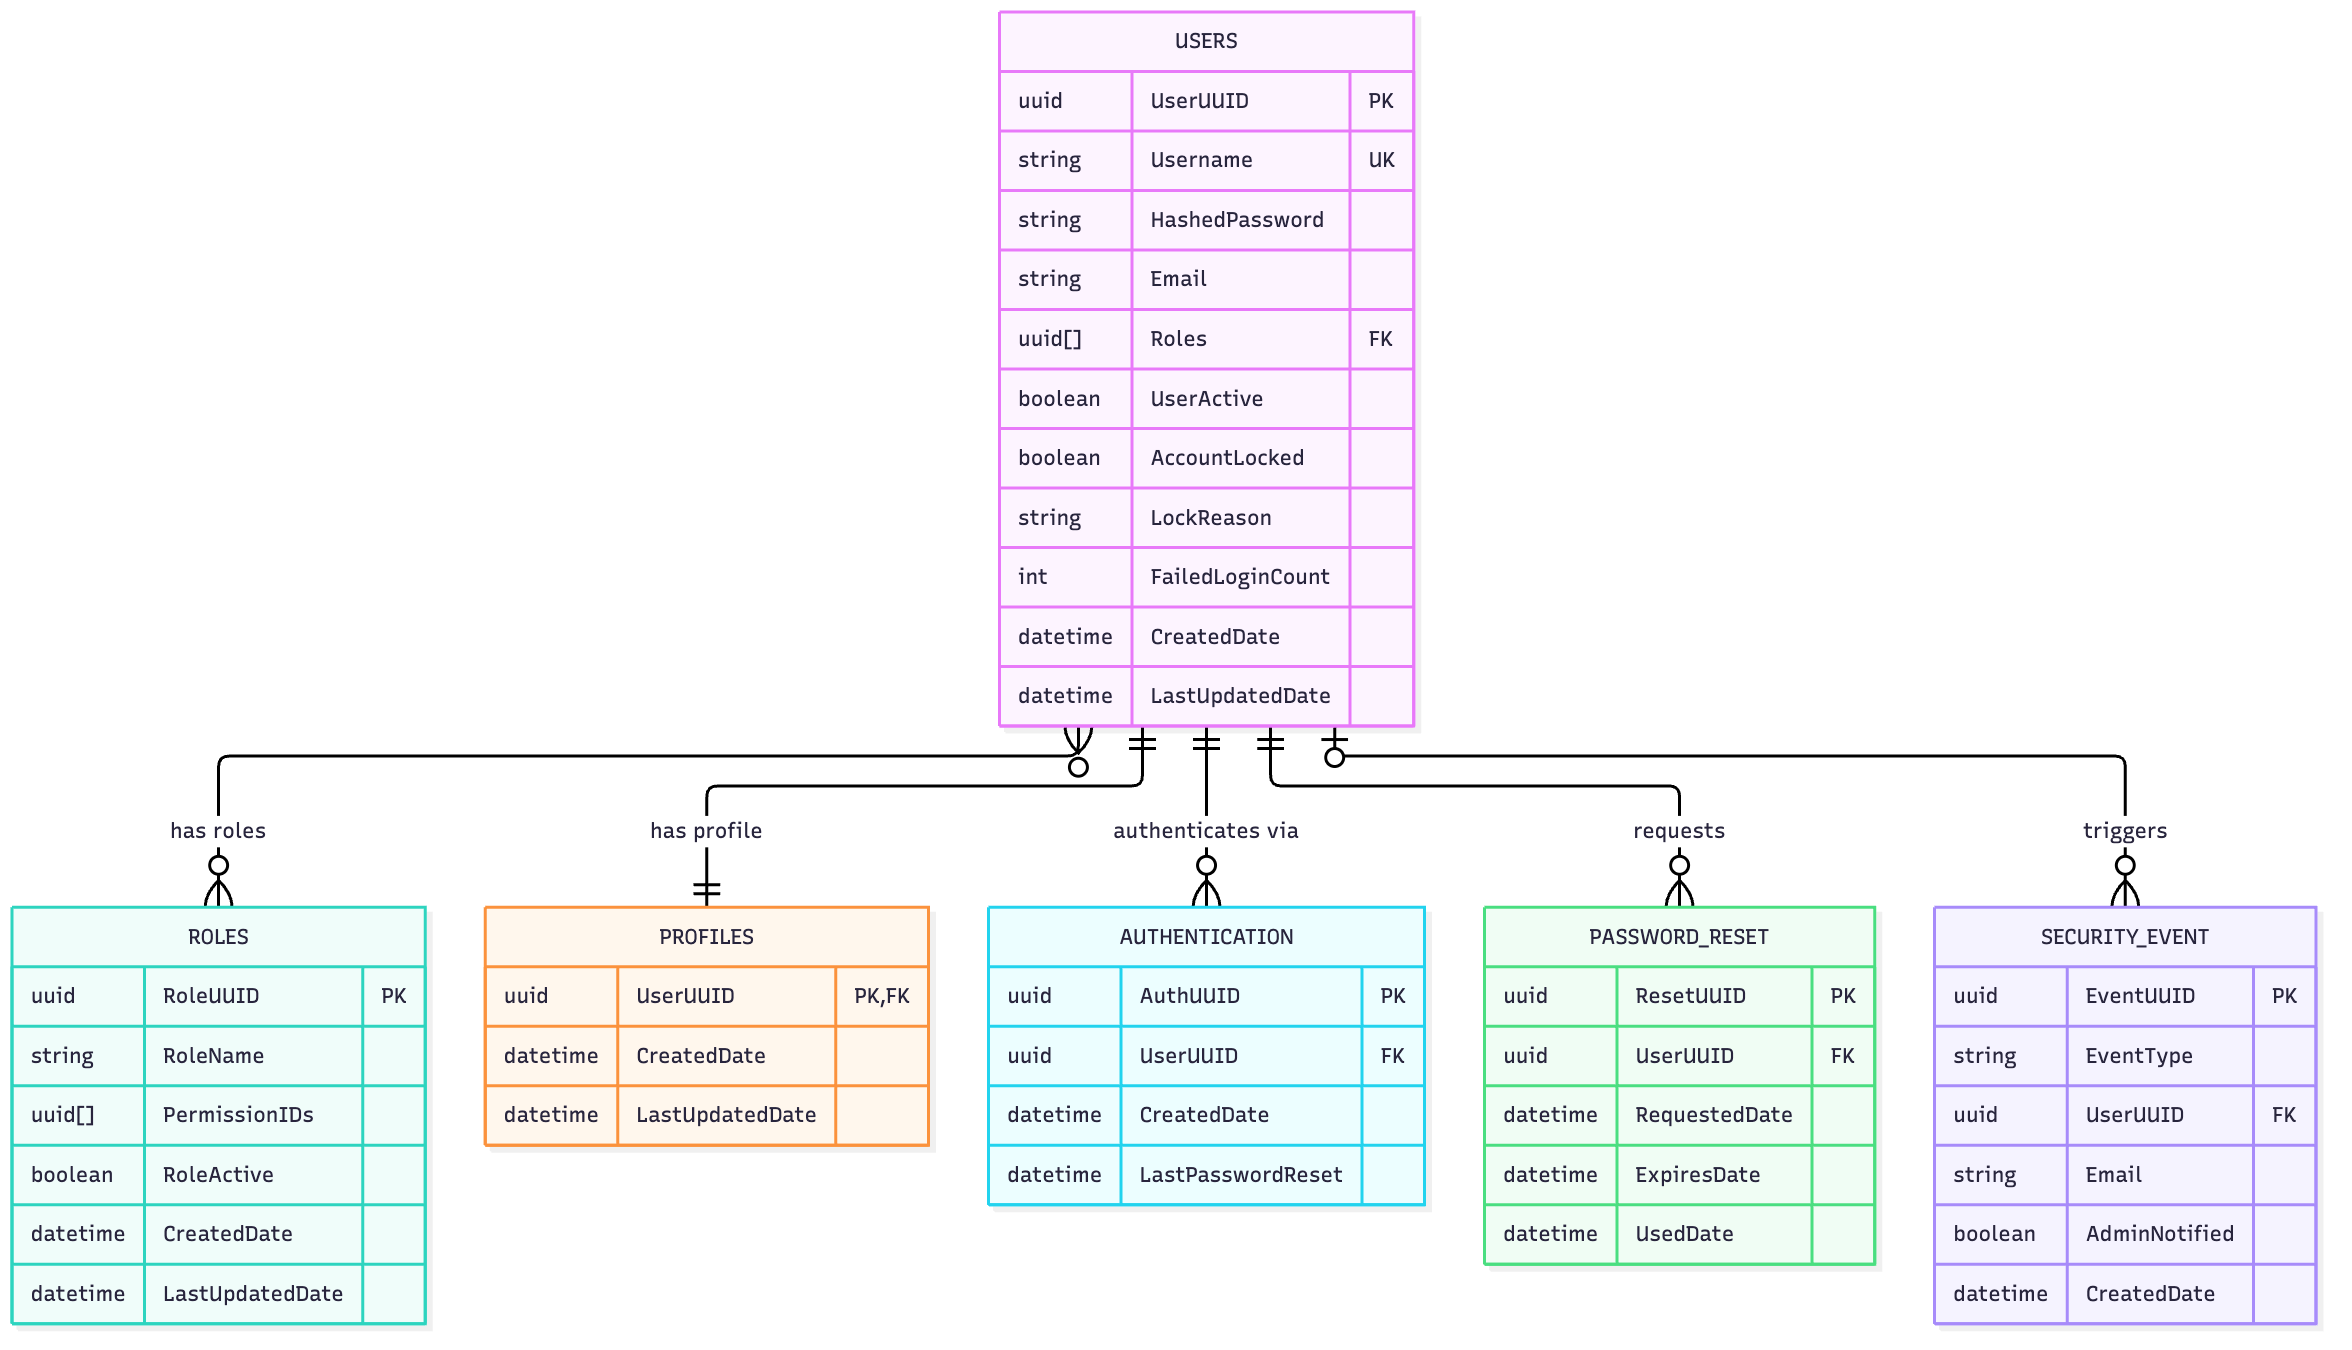
\includegraphics[width=\paperwidth]{database.png}
    \end{center}
    \end{landscape}


    \subsection{Tables}
        \begin{enumerate}[leftmargin=3\parindent]
            \item There will be a users table and a roles table.
            \item Each role will have a name, permissions, and a unique ID.
            \item A user will have a list of roles and a profile.
            \item The profile will be stored in a separate table.
            \item The users table contains a list of usernames, unique user IDs, and unique role IDs, which are used to look up the roles and profiles in their appropriate tables.
            \item The profile table associates the profiles with the unique user IDs.
            \item There will be an authentication table. Since all backend calls leverage a JWT, there must be a value that can be used to find the user for a given JWT without exposing any user information in the JWT.
            \item There will be a password reset table, which tracks every reset request so that link expiry, rate limiting, and lockouts can be enforced.
            \item There will be a security event table, which records events that require administrator notification.
        \end{enumerate}

        \subsubsection{User Table}
            \begin{enumerate}[leftmargin=3\parindent]
                \item \textbf{UserUUID} \textit{Key} Unique UUID for the user.
                \item \textbf{Username} \textit{Key} Username of the user.
                \item \textbf{HashedPassword} Hashed password for the user. This is a bcrypt hash with the salt embedded, so no separate salt column is needed.
                \item \textbf{Email} Primary email address of the user.
                \item \textbf{Roles} List of RoleIDs the user is part of.
                \item \textbf{UserActive} Can be set to false to disable a user.
                \item \textbf{AccountLocked} Set to true when the account is locked, either by failed logins or frequent password resets. An account locked by failed logins is unlocked by a forgot password reset. An account locked by frequent resets can only be unlocked by an administrator.
                \item \textbf{LockReason} Reason the account was locked, for example failed logins or frequent resets. Empty when the account is not locked.
                \item \textbf{FailedLoginCount} Number of consecutive failed logins. The account is locked at 5, and the count is cleared on a successful login or password reset.
                \item \textbf{CreatedDate} Date this entry was created.
                \item \textbf{LastUpdatedDate} Date this entry was last updated.
            \end{enumerate}

        \subsubsection{Roles Table}
            \begin{enumerate}[leftmargin=3\parindent]
                \item \textbf{RoleUUID} \textit{Key} Unique UUID for the role.
                \item \textbf{RoleName} Name of the role for display.
                \item \textbf{PermissionIDs} List of Permission IDs that the role has.
                \item \textbf{RoleActive} Can be set to false to disable a role.
                \item \textbf{CreatedDate} Date this entry was created.
                \item \textbf{LastUpdatedDate} Date this entry was last updated.
            \end{enumerate}

        \subsubsection{Profiles Table}
            \begin{enumerate}[leftmargin=3\parindent]
                \item \textbf{UserUUID} \textit{Key} UUID of the user that this profile belongs to.
                \item \textbf{CreatedDate} Date this entry was created.
                \item \textbf{LastUpdatedDate} Date this entry was last updated.
            \end{enumerate}

        \subsubsection{Authentication Table}
        The authentication table will contain at a minimum:
            \begin{enumerate}[leftmargin=3\parindent]
                \item \textbf{AuthUUID} \textit{Primary Key} Unique UUID that was generated and stored in the JWT, this is the lookup key to convert a JWT into a user.
                \item \textbf{UserUUID} \textit{Key} UUID of the user that this authentication entry belongs to.
                \item \textbf{CreatedDate} Date this entry was created.
                \item \textbf{LastPasswordReset} Last time the password was reset.
            \end{enumerate}
            All entries for a user must be deleted on logout, login session expiry, or a forgot password reset, which invalidates all of their other login sessions.

        \subsubsection{Password Reset Table}
        Every password reset request creates an entry, whether or not an email was sent, so that the reset limits can be enforced without exposing them to the user.
            \begin{enumerate}[leftmargin=3\parindent]
                \item \textbf{ResetUUID} \textit{Primary Key} Unique UUID that is included in the password reset link.
                \item \textbf{UserUUID} \textit{Key} UUID of the user that requested the reset.
                \item \textbf{RequestedDate} Date and time the reset was requested. Used to limit resets to 1 every 10 minutes and to count resets. 5 or more requests within 24 hours is a frequent reset, which locks the account and notifies an administrator.
                \item \textbf{ExpiresDate} Date and time the link expires, 4 hours after \textbf{RequestedDate}.
                \item \textbf{UsedDate} Date and time the link was clicked. Empty until clicked, and a link with a value here is no longer valid.
            \end{enumerate}
            Resets for unknown accounts have no user, so they are recorded in the Security Event table instead.

        \subsubsection{Security Event Table}
            \begin{enumerate}[leftmargin=3\parindent]
                \item \textbf{EventUUID} \textit{Primary Key} Unique UUID for the event.
                \item \textbf{EventType} Type of event, for example UnknownAccountReset, FrequentResetLock, FailedLoginLock, AccountUnlocked, or FirstAdminCreated.
                \item \textbf{UserUUID} \textit{Key} UUID of the related user. Empty when the account is unknown.
                \item \textbf{Email} Email address that was submitted, if any.
                \item \textbf{AdminNotified} Set to true once an administrator has been notified.
                \item \textbf{CreatedDate} Date this entry was created.
            \end{enumerate}
\newpage %
\section{Glossary}
    \subsection{User Facing}
    This section defines non-technical terms that may be used in this document.
    \begin{enumerate}[leftmargin=3\parindent]
        \item Student Organization -- An organization that provides support to Students, and may be comprised of Faculty, Students, or non-student members.
    \end{enumerate}

    \subsection{Technical}
    This section defines the technical terms that may be used in this document.
    \begin{enumerate}[leftmargin=3\parindent]
        \item AWS -- Amazon Web Services used for hosting the software.
        \begin{enumerate}[leftmargin=3\parindent]
            \item EC2 -- AWS Compute for running services.
            \item RDS -- AWS Database service for managing databases.
            \item S3 -- AWS File Storage
        \end{enumerate}
        \item Backend -- The portion of the software that hosts the website and database, this is the portion that the web pages reference.
        \item Docker -- Technology for deploying sites and reproducible builds.
        \item Frontend -- The web site and user facing view of the software, covers the aspect of the software running in the web browser.
        \item UUID: Universally Unique Identifier
    \end{enumerate}

    \subsection{Front End}
    \begin{enumerate}[leftmargin=3\parindent]
        \item anti-replay: anti-replay is a method of ensuring that data sent to the server cannot be sent more than once by including a token that must be sent with each request that changes.
        \item CORS: Cross-Origin Resource Sharing, this ensures that all resources served by the front-end only come from trusted domains to avoid security concerns.
        \item CSRF: Cross Site Request Forgery, this is a method of ensuring that other sites cannot impersonate the front end.
        \item JWT: JSON Web Token, used as an authentication token.
    \end{enumerate}
    \subsection{Database}
    % include the documents glossary
    \documentsGlossary

% Add the references at the end
\referencesSection[
    \item OpenAPI Specification \url{https://openapis.org}
]

\end{document}
